\documentclass{controle}
\usepackage{main}

\title{Évaluation : Fonctionnement du web et graphes}
\date{2 Février 2026}
\author{Seconde 3}

\begin{document}
\titleandname{}
\begin{questions}
\titledquestion{Usage quotidien du web}[7]
Karim se rend sur son navigateur web préféré et tape l'url suivante : \url{https://monsite.fr/home/index.html}.
\begin{parts}
\part[0,5] Donner l'exemple d'un navigateur web. 
\part[1,5] Préciser l'intérêt des différentes parties de l'url du site web visité par Karim.
\begin{subparts}
\subpart \url{https://}
\subpart \url{monsite.fr}
\subpart \url{home/index.html}
\end{subparts}
\part[1] Karim visite ensuite \url{http://mabanque.net/moncompte/}. Sa connexion est-elle sécurisée ?
\part[4] Représenter à l'aide d'un schéma un résumé du fonctionnement du navigateur de Karim, comme celui présenté en cours. On fera notamment figurer les protocoles utilisés et l'emplacement du navigateur de Karim et des serveurs nécessaires au bon fonctionnement du navigateur. On accompagnera le schéma d'un texte explicatif.
\end{parts}
\bigskip

\titledquestion{Graphes d'amitiés}[3]

On représente le graphe d'amitiés suivant :
\begin{center}
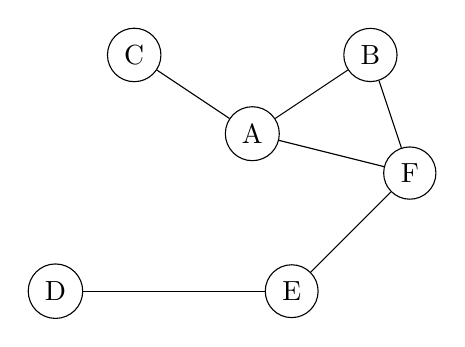
\begin{tikzpicture}
\node[circle, draw] (A) at (0,0) {A};
\node[circle, draw] (B) at (1.5,1) {B};
\node[circle, draw] (C) at (-1.5,1) {C};
\node[circle, draw] (D) at (-2.5,-2) {D};
\node[circle, draw] (E) at (0.5,-2) {E};
\node[circle, draw] (F) at (2,-0.5) {F};

\draw (A) -- (B);
\draw (B) -- (F);
\draw (F) -- (A);
\draw (F) -- (E);
\draw (E) -- (D);
\draw (C) -- (A);
\end{tikzpicture}
\end{center}
\begin{parts}
\part[1] Combien y a-t-il d'arêtes sur ce graphe ?
\part[2] Donner le degré de chacun des sommets. Quelle personne est la plus populaire sur ce graphe d'amitiés ?
\end{parts}
\end{questions}
\end{document}